\documentclass[coverwidth=151mm, 
	       coverheight=216mm,
               spinewidth=6mm,
               bleedwidth=2mm,
               marklength=1mm,
               12pt]{bookcover}
\usepackage[osf]{coelacanth}

\begin{document}
\begin{bookcover}
\bookcovercomponent{normal}{front}{

\vspace{10mm}

\begin{center}
\fontsize{40}{48}\selectfont Menschen \& Magie

\large{Geheimes Wissen}

\vspace{5mm}

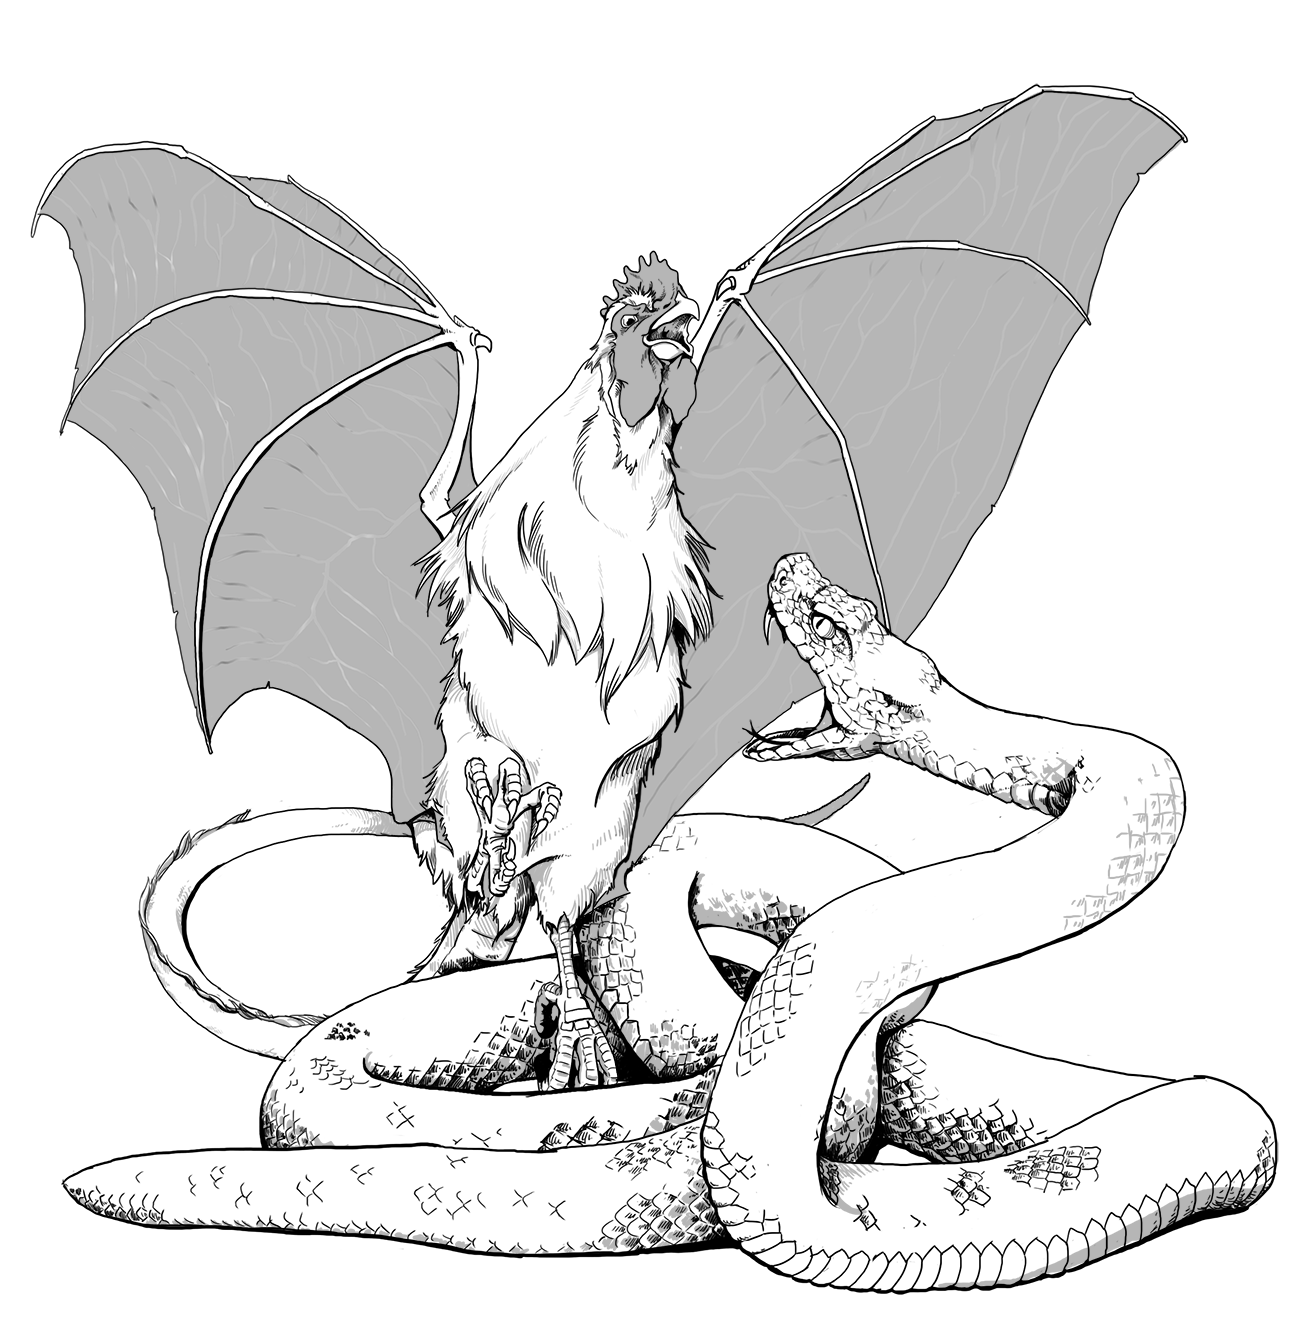
\includegraphics[height=120mm]{../img/DnD-Cockatrice.png}

\vspace{10mm}


\includegraphics[height=1.9cm]{../img/logo.png}
\end{center}
}
\bookcovercomponent{center}{spine}{
\rotatebox[origin=c]{270}{Menschen \& Magie - Geheimes Wissen}
\vfill
\includegraphics[width=5mm]{../img/wb.png}
}

\end{bookcover}
\end{document}
